\begin{frame}
\begin{block}{examples of initial and final objects}
For example, in \textit{Sets} the empty set $\emptyset$ is the unique
initial object and any {\it singleton} set, a set with one element,
is a final object.
\end{block}

\begin{block}{{\it external}/generalized elements}
\centering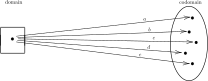
\includegraphics[width=0.8\framewidth]{fig/points.pdf}
\end{block}
\end{frame}